\makeheading{2020-03-27}
\section{Non-planar Graphs}
In a planar drawing of $ G=(V,E) $ with set of faces $ F $,
and $ G $ connected,
\begin{itemize}
    \item $ |V|-|E|+|F|=2 $
    \item $ \sum\limits_{f\in F}\deg(f)=2|E| $
\end{itemize}
We will combine these to prove that various graphs
(such as $ K_5 $) are not planar.


\begin{Proposition}{}{}
    In any planar drawing of a graph that is not a tree,
    every face has a boundary walk that contains
    (the edges of) a cycle.
\end{Proposition}

Therefore, the boundary walk of every face has
length $ \geqslant 3 $ (unless the graph has $ \leqslant $ 1 edge).
It follows that, if $ G $ is a connected plane graph with $ \geqslant 2 $
edges, then in any drawing of $ G $, each face has degree $ \geqslant 3 $.


\begin{Proposition}{}{}
    In a drawing of a connected plane graph $ G=(V,E) $
    with $ |E|\geqslant 2 $, and set $ F $ of faces, we have
    \[ |F|\leqslant \frac{2}{3}|E| \]
\end{Proposition}

\begin{Proof}{}{}
    By Handshaking for Faces,
    \begin{align*}
        2|E|
         & =\sum\limits_{f\in F}\deg(f) \\
         & \geqslant 3|F|
    \end{align*}
    where the last inequality holds because each face has degree $ \geqslant 3 $.
    Thus,
    \[ |F|\leqslant \frac{2}{3}|E| \]
\end{Proof}


\begin{Lemma}{}{bound_edge}
    If $ G=(V,E) $ is a connected planar graph with $ |V|\geqslant 3 $,
    then
    \[ |E|\leqslant 3|V|-6 \]
\end{Lemma}

\begin{Proof}{}{}
    We know that $ |V|-|E|+|F|=2 $ and $ |F|\leqslant \frac{2}{3} |E| $,
    where $ F $ is the set of faces in some planar drawing of $ G $.
    Combining, yields
    \[ 2=|V|-|E|+|F|\leqslant |V|-|E|+\frac{2}{3}|E| \]
    \[ \implies 2\leqslant |V|-\frac{1}{3} |E| \]
    \[ \implies |E|\leqslant 3|V|-6 \]
\end{Proof}


\begin{Corollary}{}{}
    The graph $ K_5 $ is not planar.
\end{Corollary}

\begin{Proof}{}{}
    $ K_5 $ has $ 5 $ vertices and $ 10 $ edges, but
    \[ 10\nleqslant 3\cdot 5-6=9 \]
\end{Proof}
As we could see, $ K_5 $ has too many edges to be planar.
If we removed one edge, we could get a planar graph:

\begin{figure}[H]
    \centering
    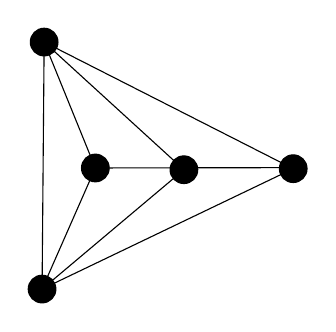
\begin{tikzpicture}[x=0.75pt,y=0.75pt,yscale=-1,xscale=1]
        %uncomment if require: \path (0,300); %set diagram left start at 0, and has height of 300

        %Shape: Circle [id:dp41001528797573905] 
        \draw  [fill={rgb, 255:red, 0; green, 0; blue, 0 }  ,fill opacity=1 ] (178.67,100.33) .. controls (178.67,96.65) and (181.65,93.67) .. (185.33,93.67) .. controls (189.02,93.67) and (192,96.65) .. (192,100.33) .. controls (192,104.02) and (189.02,107) .. (185.33,107) .. controls (181.65,107) and (178.67,104.02) .. (178.67,100.33) -- cycle ;
        %Shape: Circle [id:dp6741334404747168] 
        \draw  [fill={rgb, 255:red, 0; green, 0; blue, 0 }  ,fill opacity=1 ] (221.33,101.17) .. controls (221.33,97.48) and (224.32,94.5) .. (228,94.5) .. controls (231.68,94.5) and (234.67,97.48) .. (234.67,101.17) .. controls (234.67,104.85) and (231.68,107.83) .. (228,107.83) .. controls (224.32,107.83) and (221.33,104.85) .. (221.33,101.17) -- cycle ;
        %Shape: Circle [id:dp8243036373436615] 
        \draw  [fill={rgb, 255:red, 0; green, 0; blue, 0 }  ,fill opacity=1 ] (274,100.67) .. controls (274,96.98) and (276.98,94) .. (280.67,94) .. controls (284.35,94) and (287.33,96.98) .. (287.33,100.67) .. controls (287.33,104.35) and (284.35,107.33) .. (280.67,107.33) .. controls (276.98,107.33) and (274,104.35) .. (274,100.67) -- cycle ;
        %Shape: Circle [id:dp12724886477248498] 
        \draw  [fill={rgb, 255:red, 0; green, 0; blue, 0 }  ,fill opacity=1 ] (154,39.67) .. controls (154,35.98) and (156.98,33) .. (160.67,33) .. controls (164.35,33) and (167.33,35.98) .. (167.33,39.67) .. controls (167.33,43.35) and (164.35,46.33) .. (160.67,46.33) .. controls (156.98,46.33) and (154,43.35) .. (154,39.67) -- cycle ;
        %Shape: Circle [id:dp7769733828255948] 
        \draw  [fill={rgb, 255:red, 0; green, 0; blue, 0 }  ,fill opacity=1 ] (153,158.67) .. controls (153,154.98) and (155.98,152) .. (159.67,152) .. controls (163.35,152) and (166.33,154.98) .. (166.33,158.67) .. controls (166.33,162.35) and (163.35,165.33) .. (159.67,165.33) .. controls (155.98,165.33) and (153,162.35) .. (153,158.67) -- cycle ;
        %Straight Lines [id:da6246549221396057] 
        \draw    (160.67,39.67) -- (280.67,100.67) ;
        %Straight Lines [id:da09776853172786704] 
        \draw    (185.33,100.33) -- (280.17,100.17) ;
        %Straight Lines [id:da09893264834575233] 
        \draw    (159.67,158.67) -- (160.67,39.67) ;
        %Straight Lines [id:da815821795444068] 
        \draw    (159.67,158.67) -- (280.67,100.67) ;
        %Straight Lines [id:da1808916613862651] 
        \draw    (159.67,158.67) -- (228,101.17) ;
        %Straight Lines [id:da8225006703405966] 
        \draw    (160.67,39.67) -- (185.33,100.33) ;
        %Straight Lines [id:da637574437134229] 
        \draw    (185.33,100.33) -- (159.67,158.67) ;
        %Straight Lines [id:da1168536310589865] 
        \draw    (228,101.17) -- (160.67,39.67) ;




    \end{tikzpicture}

    \caption{$ K_5-e $}
\end{figure}


\begin{Proposition}{}{}
    If $ G $ is connected graph on $ \geqslant 3 $ vertices
    with $ |E|\geqslant 3|V|-5 $, then $ G $ is non-planar.
\end{Proposition}

\begin{Proof}{}{}
    Contrapositive of~\Cref{lem:bound_edge}.
\end{Proof}
We can't use this proposition to prove $ K_{3,3} $ is non-planar.

\textbf{Recall} The boundary of any face contains a cycle (in a plane drawing
of a graph that is not a tree).


\begin{Corollary}{}{}
    In a plane drawing of a graph $ G=(V,E) $ with
    $ |V|\geqslant 3 $ and set of faces $ F $, such that
    $ G $ has no $3$-cycle every face
    has degree $ \geqslant 4 $.
\end{Corollary}



\begin{Corollary}{}{}
    In a graph $ G $ as above,
    \[ |F|\leqslant \frac{1}{2} |E| \]
\end{Corollary}

\begin{Proof}{}{}
    Handshaking with Faces gives,
    \[ 2|E|=\sum\limits_{f\in F}\deg(f)\geqslant 4|F| \]
\end{Proof}


\begin{Corollary}{}{}
    If $ G=(V,E) $ is planar and connected,
    has $ \geqslant 3 $ vertices, and has no
    $ 3 $-cycle, then
    \[ |E|\leqslant 2|V|-4 \]
\end{Corollary}

\begin{Proof}{}{}
    \[ 2=|V|-|E|+|F|\leqslant |V|-|E|+\frac{1}{2} |E| \]
    \[ 2\leqslant |V|-\frac{1}{2} |E|\implies |E|\leqslant 2|V|-4 \]
\end{Proof}


\begin{Corollary}{}{}
    $ K_{3,3} $ is non-planar.
\end{Corollary}

\begin{Proof}{}{}
    $ K_{3,3} $ has $ |V|=6 $ and $ |E|=9 $, but
    \[ 9\nleqslant 2\cdot 6-4=8 \]
\end{Proof}

$ K_5 $ and $ K_{3,3} $ are non-planar, so are all their super graphs.

\begin{figure}[H]
    \centering
    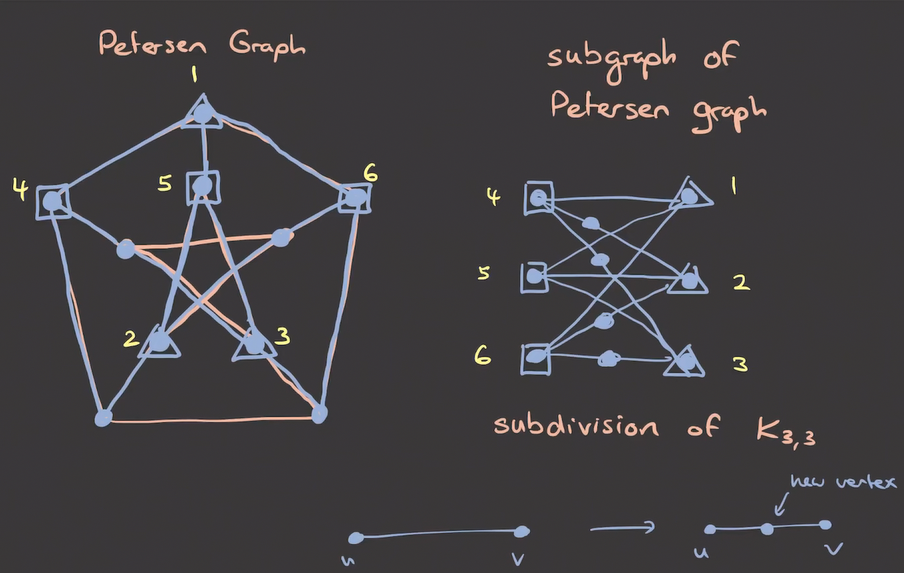
\includegraphics[scale=0.8]{petersen.png}
\end{figure}


\begin{Definition}{}{}
    If $ uv $ is an edge in a graph $ G $, the graph $ G^{\prime} $
    is obtained by \textbf{\emph{subdividing}} the edge $ uv $
    has vertex set
    \[ V(G)\cup \{x\} \]
    where $ x $ is a new vertex, and edge set
    \[ (E(G)\setminus \{uv\})\cup \{ux,vx\} \]
\end{Definition}



\begin{Definition}{}{}
    A \textbf{\emph{subdivision}} of a graph $ G $ is any graph
    obtained from $ G $ by repeatedly ($ \geqslant 0 $) subdividing edges.
\end{Definition}



\begin{Proposition}{}{}
    If $ H $ is a non-planar graph, then every subdivision of $ H $
    is also non-planar.
\end{Proposition}

\begin{Proof}{}{}
    Any planar drawing of a subdivision of $ H $ would give rise to
    a plane drawing of $ H $.
\end{Proof}


\begin{Corollary}{}{}
    If $ H $ is a non-planar graph, and $ G $ is a graph
    having a subdivision of $ H $ as a subgraph, then $ G $
    is non-planar.
\end{Corollary}


\section{Kuratowski's Theorem}

\begin{Theorem}{Kuratowski's Theorem}{Kuratowski}
    A graph $ G $ is planar if and only if $ G $ does not
    contain a subdivision of $ K_5 $ or $ K_{3,3} $.
\end{Theorem}

\begin{Proof}{}{}
    Beyond the scope of this course. However, the proof is covered in
    CO 342.
\end{Proof}


\begin{Corollary}{}{}
    If $ G $ is non-planar, then $ G $ must contain
    (as a subgraph) a subdivision of either $ K_5 $ or $ K_{3,3} $.
\end{Corollary}

\begin{Proof}{}{}
    Contrapositive of~\Cref{thm:Kuratowski}.
\end{Proof}


\begin{Theorem}{}{}
    For any topological surface, there is a finite list of graphs that behave
    like $ K_{3,3} $ and $ K_5 $ do for the plane.
\end{Theorem}

